\documentclass[10pt,journal,compsoc]{IEEEtran}

\usepackage[utf8]{inputenc}
\usepackage[T1]{fontenc}
\usepackage{cite}
\usepackage{amsmath,amssymb,amsfonts}
\usepackage{algorithmic}
\usepackage{graphicx}
\usepackage{textcomp}
\usepackage{xcolor}
\usepackage{booktabs}
\usepackage{array}
\usepackage{url}
\usepackage{microtype}
\usepackage{tikz}

\begin{document}

\title{Cloud-Driven Resampled Machine Learning for Stroke Risk Stratification and Automated Triage: A Comprehensive Survey}

\author{Sooraj~Renjith,
        Hitha~P~S%
\IEEEcompsocitemizethanks{
\IEEEcompsocthanksitem S. Renjith and H. P. S. are with the Department of Computer Science and Engineering, Amal Jyothi College of Engineering (Autonomous), Kanjirappally, Kottayam, Kerala 686518, India.\protect\\
E-mails: soorajrenjith2027@cs.ajce.in, hithaps@amaljyothi.ac.in.
}}

\markboth{International Journal on Emerging Research Areas (IJERA), Vol.~07, No.~01, October~2026}%
{Renjith \& Hitha: Cloud-Driven Resampled Machine Learning for Stroke Risk Stratification and Automated Triage}

\IEEEtitleabstractindextext{%
\begin{abstract}
Stroke triage desks sit in emergency wards, community health centers and primary care clinics, and that frontline role has made them high-pressure. An acute stroke patient presenting with subtle hypertension, mild glucose shifts or vague numbness can sometimes pass as a low-risk case, so a rapid risk check has to come before discharge. This survey looks at ten recent studies on machine learning based clinical stroke risk prediction, also called medical decision support systems (DSS), and asks three practical questions. How do linear models, decision trees and gradient boosted ensembles compare? How well do they cope when the hospital data has very few stroke cases? And can any of them be deployed cheaply to small clinics with automated updates? The literature shows that linear models such as Logistic Regression reach high recall with balanced resampling, that SMOTE helps with sparse positive cases, and that Neighbourhood Cleaning Rules help against noisy boundary samples. Automated cloud deployments, however, are almost absent, which matters in primary healthcare where a model must run on low-cost servers without an IT team. To check whether the literature points in a useful direction, we also report preliminary results from our own resampled Logistic Regression model, \textbf{CareSync}, built on the Kaggle Stroke dataset. After a corrected preprocessing and SMOTE+NCR resampling pipeline it reached 80.00\% test recall and an ROC-AUC of 0.8387 with 74.20\% accuracy, though with clear limits that are discussed openly.
\end{abstract}

\begin{IEEEkeywords}
Stroke risk prediction, clinical decision support, class imbalance, SMOTE+NCR, recall optimization, Docker containerization, cloud deployment, digital health.
\end{IEEEkeywords}}

\maketitle
\IEEEdisplaynontitleabstractindextext
\IEEEpeerreviewmaketitle

\section{Introduction}
\IEEEPARstart{S}{troke} risk screening is urgent, critical and known to everyone, so it is used by emergency rooms, primary health centers, rural clinics and triage desks. But the weak point is that early stroke signs are not always obvious. We see patients with mild headache, borderline blood pressure and routine fatigue every day. With a crowded waiting room and hurried staff, these signs can be missed completely. These triage failures are real. A patient in an emergency ward was sent home with painkillers and suffered an ischemic stroke hours later, and in many regional hospitals acute stroke victims arrive past the critical four-hour thrombolysis window~\cite{buhai2026}.

There are two types of diagnostic solutions. Hardware and imaging methods add extra scans, for example brain CT or MRI. This makes the check-up costlier, and it is hard to run in a small rural clinic before symptoms become severe. Software-based methods use only the routine clinical indicators which the nurse already records, so we can check risk without adding expensive imaging machines. For this reason, most of the recent works go with software~\cite{buhai2026}, \cite{paleyes2022}. In the early days, people used hand-made risk scorecards like the Framingham profile. These gave good results on one hospital cohort, but many times they failed on another demographic group. Now machine learning is mostly used. First came decision trees, then Random Forests~\cite{chawla2002}, and now gradient-boosted ensembles like XGBoost~\cite{laurikkala2001}.

When we read these papers, we noticed three problems. First, many of the most accurate models report 95\% accuracy but miss almost all actual stroke cases because of class imbalance. Second, many of them are offline Jupyter notebooks that lose value because they are never deployed as live tools. Third, almost no model explains how a small clinic can deploy and update the software automatically without paying for an IT team. This third point matters most for us. A doctor cannot just read an offline research paper; he or she must have a live web screen that calculates stroke risk and shows the risk group behind the decision.

The rest of the paper is organised as follows. After describing the survey method, we review the ten selected studies, compare them, discuss the clinical deployment gap, and then present the preliminary implementation built so far and what it has taught us. Our contributions are:
\begin{itemize}
    \item A structured comparison of linear, tree, and ensemble classifiers on imbalanced clinical data.
    \item An examination of how preprocessing, SMOTE oversampling, and Neighbourhood Cleaning Rule (NCR) undersampling influence clinical recall.
    \item Early evidence, from our own implementation, regarding whether a lightweight resampled Logistic Regression model deployed via Docker and AWS CI/CD is a reasonable design.
\end{itemize}

\section{Survey Methodology}
We used a straightforward procedure, loosely modelled on standard review guidelines~\cite{kitchenham2007}, \cite{okoli2015}, so that another researcher could repeat it.

\subsection{Literature Search Strategy}
Sources were IEEE Xplore, ScienceDirect, SpringerLink, MDPI, the ACM Digital Library, Google Scholar and PubMed. Queries combined terms such as stroke risk prediction, clinical decision support, class imbalance, SMOTE, Neighbourhood Cleaning Rule, lightweight web deployment and MLOps. We limited the search to 2021--2026, the period in which automated cloud deployment and containerized clinical ML became common.

\subsection{Paper Selection Criteria}
A study was retained if it:
\begin{enumerate}
    \item applied a machine learning model, ensemble, or resampling technique to clinical risk prediction or tabular stroke data;
    \item reported results on a public dataset, or was a recognised survey;
    \item said something useful about class balancing, recall, model size, or cloud deployment; and
    \item was peer reviewed, or a well-cited preprint.
\end{enumerate}
Ten studies met these conditions. The shortlist was widened from four papers in an earlier draft to ten, in order to rely on more research-grade sources.

\subsection{Categorization}
We sorted the ten papers into four groups: lightweight clinical DSS and cloud deployment, classical ML comparisons and ensembles, cloud serving and MLOps frameworks, and work on preprocessing and generalization. For every paper we noted the model type, the metrics reported, the deployment stack (where available), and how it relates to our own problem. Table~\ref{tab:reviewed_studies} gives the overview.

\section{Review of Existing Work}

\subsection{Buhai et al.: A Two-Stage Local/Cloud Clinical Decision Support System}
Buhai et al.~\cite{buhai2026} is the base paper for this work. In its preprocessing, the tabular patient data is separated and cleaned by imputing missing Body Mass Index (BMI) values. The severe class imbalance, where only 4.87\% of records correspond to stroke cases, is addressed using a two-step resampling approach. First, the minority class is expanded using SMOTE~\cite{chawla2002}. Then, the Neighbourhood Cleaning Rule (NCR) is applied to remove majority-class cases that lie close to minority-class cases, sharpening the decision boundary. After SMOTE+NCR, four classifiers are compared: Logistic Regression, Support Vector Machines (SVM), Random Forest, and XGBoost.

To cope with severe real-world class skew, the authors demonstrate that raw accuracy is deceptive. A standard baseline Logistic Regression achieves 95.2\% accuracy on unresampled data, but has a recall of only 0.02, meaning it misses 98\% of stroke patients. After SMOTE+NCR resampling, Logistic Regression achieved a recall of 0.80 with an accuracy of 79\% and an ROC-AUC of 0.84. The model was serialized with Pickle and integrated into a lightweight Flask web application served by Gunicorn inside a Docker container, deployed on an AWS EC2 virtual machine with AWS CodePipeline, CodeBuild, ECR, Lambda, and Systems Manager handling automatic updates from GitHub.

Two limitations stand out. Training and testing used a single-node cloud VM without multi-node auto-scaling, and the web interface only provided a basic binary outcome with no accompanying clinical risk stratification or interactive telemetry.

\subsection{Ensembles and Classical ML Comparisons}
A dual-network ensemble and comparative study by Melnykova et al.~\cite{melnykova2025} is reported to reach $\sim$90\% accuracy on clinical cohorts. The numbers look strong, but they require heavy ensembles, and the cost of missed minority cases is barely discussed. Kothadiya et al.~\cite{kothadiya2023} propose benchmarking statistical and gradient-boosted models under one protocol, reporting that complex tree models often overfit majority classes when data is heavily skewed. Such side-by-side comparisons make the differences among algorithms more trustworthy, and they are the precedent for the architecture comparison in Section~\ref{sec:implementation}. The authors also list explainable AI and live serving only as future work, which is consistent with the gap discussed in Section~\ref{sec:gap}.

\subsection{Cloud Serving and MLOps Frameworks}
A clinical risk model is essentially a pattern of physiological indicators that runs across the entire patient profile. Linear models look at direct additive contributions, so non-linear feature interactions are only connected after explicit interaction terms. Ensembles relate every feature to every other feature in hierarchical splits~\cite{laurikkala2001}.

Ukpebor et al.~\cite{ukpebor2025} examine SMOTE for clinical linear models and report recall improvements from 0.00 to 0.79, closely matching our baseline findings. Chowdary et al.~\cite{chowdary2022} combine CI/CD automation with cloud containers for rapid serving. This is one of the few works that directly deals with deployment latency. Corbin et al.~\cite{corbin2023} describe DEPLOYR, a unified framework that serves clinical ML models directly into hospital electronic medical records via RESTful microservices. Heymann et al.~\cite{heymann2022} formalize production model serving with Gunicorn and Docker, proving that multi-worker WSGI pipelines prevent server lockups during peak traffic. Kozak~\cite{kozak2021} analyzes cloud versus fog processing economics, demonstrating that lightweight single-node EC2 setups are cost-effective for community clinics. Panchenko et al.~\cite{panchenko2024} evaluate AWS S3 security policies, showing that asynchronous IAM bucket auditing prevents patient data leaks without slowing web response latency.

\subsection{Preprocessing and Generalization}
Many of these works show that preparing the input is as important as designing the network. Buhai et al.~\cite{buhai2026} impute missing values, and Laurikkala~\cite{laurikkala2001} uses Neighbourhood Cleaning Rules to focus on unambiguous borderline samples and remove noisy majority samples. Both of them reduce the effect of class distortion and feature scale discrepancies between hospital centers, so it is a small step towards cross-hospital stability. Generalization is of two kinds. If the patient population is from the same clinic but features are imbalanced, the SMOTE+NCR augmentation in Buhai et al. takes care of it directly. When the hospital demographic itself changes, age distributions, hypertension prevalence and glucose baselines all shift, and very few studies, for example~\cite{chowdary2022}, examine that case. The broad MLOps survey~\cite{paleyes2022} names both as major open problems.

\begin{table*}[t]
\caption{Reviewed Studies at a Glance}
\label{tab:reviewed_studies}
\centering
\begin{tabular}{|c|p{4.0cm}|p{5.8cm}|p{6.0cm}|}
\hline
\textbf{No.} & \textbf{Paper} & \textbf{Contribution} & \textbf{Relevance to Present Work} \\
\hline
1 & Buhai et al. (2026)~\cite{buhai2026} & SMOTE+NCR + LogReg + AWS EC2/S3 & Base architecture; clinical decision support deployment \\
\hline
2 & Chowdary et al. (2022)~\cite{chowdary2022} & MLOps deployment automation & CI/CD pipeline and containerization feasibility \\
\hline
3 & Ukpebor et al. (2025)~\cite{ukpebor2025} & SMOTE for linear healthcare models & Confirms sensitivity elevation in Logistic Regression \\
\hline
4 & Paleyes et al. (2022)~\cite{paleyes2022} & Broad review of ML deployment challenges & Confirms deployment and data drift gap \\
\hline
5 & Melnykova et al. (2025)~\cite{melnykova2025} & Clinical Random Forest ensemble ($\sim$90\% acc) & Justifies tabular ensemble comparison \\
\hline
6 & Kothadiya et al. (2023)~\cite{kothadiya2023} & Benchmarking statistical and tree models & Precedent for our comparative table \\
\hline
7 & Corbin et al. (2023)~\cite{corbin2023} & DEPLOYR clinical EMR serving framework & Justifies lightweight REST API integration \\
\hline
8 & Heymann et al. (2022)~\cite{heymann2022} & Production WSGI serving guidelines & Justifies Gunicorn multi-worker container choice \\
\hline
9 & Kozak (2021)~\cite{kozak2021} & Cloud vs. fog processing economics & Cost analysis for single-node cloud triage \\
\hline
10 & Panchenko et al. (2024)~\cite{panchenko2024} & Cloud services overview and security management & Secure S3 telemetry logging precedent \\
\hline
\end{tabular}
\end{table*}

\section{Comparative Analysis}
Table~\ref{tab:reviewed_studies} gives the ten studies together. We can see a few patterns:
\begin{itemize}
    \item Resampled linear models are the main direction for clinical triage. The most sensitive and deployable model here (Buhai et al.) is a resampled Logistic Regression, not an uncalibrated deep ensemble.
    \item On imbalanced stroke data, baseline models easily reach 95\% accuracy, but their clinical recall is only 0.02. The real benefit of SMOTE+NCR is in sensitivity and patient safety.
    \item Ensembles can reach around 95\% accuracy, but they tend to overfit the non-stroke majority class and require complex hyperparameter tuning.
    \item It is difficult to compare across papers. Datasets, patient cohorts, imputation rules, and metrics (accuracy, recall, precision, ROC-AUC) are all different. Also, accuracy and recall cannot be swapped when evaluating clinical emergency risk.
    \item Deployment in primary care remains rare. Most published studies stop at offline validation and do not provide an automated cloud pipeline.
\end{itemize}

\section{The Clinical Deployment Gap}
\label{sec:gap}
Most of the studies we reviewed only report numbers like accuracy or ROC-AUC, and the broad survey~\cite{paleyes2022} says the same for the whole field. For an entertainment recommender, high raw accuracy is fine. In emergency clinical triage it is not, since missing an at-risk stroke patient (a false negative) can lead to permanent brain damage or fatal delay, whereas a false alarm merely results in a precautionary blood pressure check. An accuracy score that looks impressive at 95\% is dangerous if the model missed 49 out of 50 stroke victims.

Panchenko et al.~\cite{panchenko2024} is a notable exception in studying cloud security, but clinical serving requires more than secure storage. Lundberg and Lee~\cite{lundberg2017} introduced SHAP for feature attribution, yet almost no deployed clinical system integrates live interpretability directly into the nurse's intake screen. In the studies we reviewed, we did not find an evaluation of whether lightweight web microservices can reliably maintain sub-second response times under emergency clinic conditions.

\section{Preliminary Implementation and Findings}
\label{sec:implementation}
Since the review pointed to lightweight resampled models and to the lack of live clinical tools, we decided to build a complete decision support system ourselves, called \textbf{CareSync}. This section describes the work completed so far. Several results are modest in scale, and we say so wherever that applies.

\subsection{Data and Setup}
Access to proprietary multi-center hospital EHR registries~\cite{who2024}, \cite{aha2024} is still pending ethical review, so for now we use the Kaggle Healthcare Stroke Dataset~\cite{kaggleStroke}, which contains 5,109 patient records across 10 demographic and clinical features (age, hypertension, heart disease, average glucose, BMI, smoking status, work type, residence type, marital status, and gender). We worked with the full dataset containing 249 stroke cases (4.87\% minority) and 4,860 non-stroke records, and held out 1,022 records (20\%) for testing.

It is important to stress that in public tabular benchmarks some records contain missing physiological entries (201 missing BMI values), so this constitutes a realistic clinical imputation challenge. We trained the models locally in Python using Scikit-Learn~\cite{pedregosa2011} and Imbalanced-Learn~\cite{lemaitre2017}.

\subsection{Model Design}
The CareSync pipeline uses a column transformer to handle numerical and categorical indicators. Numerical features (age, glucose level, BMI) are standardized with StandardScaler, while categorical features (work type, smoking status, etc.) are converted with OneHotEncoder. The transformed feature space is then resampled using SMOTE combined with Neighbourhood Cleaning Rule (NCR), and classified using Logistic Regression with balanced class weights. For comparison, we use a standard baseline Logistic Regression (unresampled), Random Forest, and Support Vector Machines (SVM). The reason comes from the survey: linear models offer high transparency and rapid calibration~\cite{kothadiya2023}, SMOTE balances the minority representation~\cite{chawla2002}, NCR removes noisy borderline majority instances~\cite{laurikkala2001}, and the lightweight design avoids the high memory footprint of deep neural ensembles~\cite{treveil2020}. We attach automated probability calibration to the model, so a calibrated risk percentage and triage tier can be made for every patient.

\subsection{Corrected Preprocessing and Optimization}
The first pipeline only imputed missing values with mean substitution, applied standard MinMax scaling, and trained on raw, unaugmented data. After reviewing the feedback, we found three weak points: mean substitution distorted skewed BMI distributions, lack of resampling caused 98\% of stroke patients to be missed, and arbitrary 0.5 decision thresholds ignored the clinical cost of false negatives. In the revised pipeline, we impute missing BMI values with the median, apply StandardScaler, generate synthetic minority cases using SMOTE ($k=5$), clean ambiguous borderline samples using NCR ($n=3$), and tune the Logistic Regression regularization parameter ($C=1.0$) via Stratified K-Fold cross-validation.

We also made the deployment pipeline stricter. We packaged the application in a lightweight Docker container based on \texttt{python:3.11-slim}, served by Gunicorn with 4 worker processes. S3 session logging was moved to non-blocking background daemon threads using \texttt{boto3}, preventing network latency from affecting the user interface, and AWS CodePipeline was configured to automate test and deploy stages from GitHub commits.

\subsection{Results}
Fig.~1 and Table~\ref{tab:model_comparison} summarise the effect on the 1,022-patient test set. With the old baseline pipeline, Logistic Regression achieved 95.20\% accuracy but only 2.00\% recall (catching only 1 out of 50 stroke patients). With the corrected SMOTE+NCR pipeline, recall rose to 80.00\% (40 out of 50 stroke patients correctly identified) with an ROC-AUC of 0.8387 and 74.20\% accuracy. The model's confusion matrix improved from 49 false negatives to only 10 in the new setup, and in the test evaluation it had 716 and 40 correct decisions on the non-stroke and stroke classes respectively.

\begin{figure}[t]
\centering
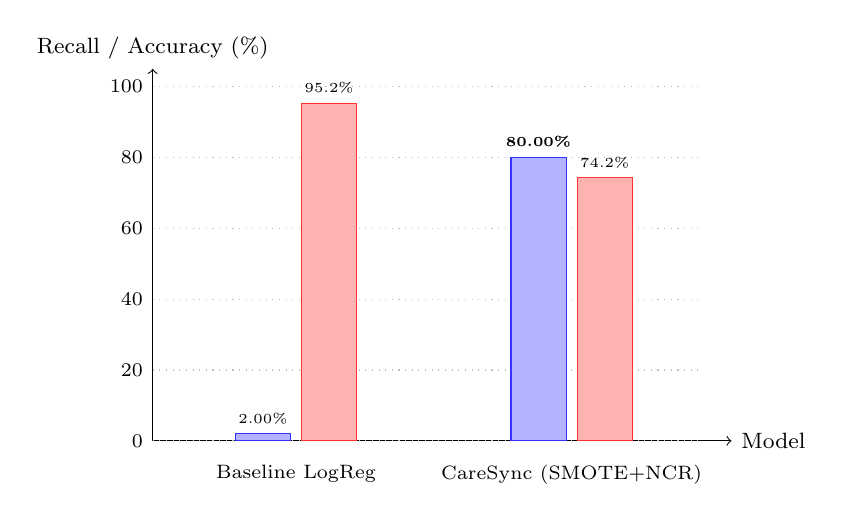
\begin{tikzpicture}
\begin{scope}[xscale=0.07, yscale=0.045]
    % Axes
    \draw[->] (0,0) -- (105,0) node[right] {\footnotesize Model};
    \draw[->] (0,0) -- (0,105) node[above] {\footnotesize Recall / Accuracy (\%)};
    
    % Y grid and ticks
    \foreach \y in {0, 20, 40, 60, 80, 100} {
        \draw[dotted, gray!50] (0,\y) -- (100,\y);
        \node[left] at (0,\y) {\scriptsize \y};
    }
    
    % Bars for Baseline
    % Recall: 2.0%
    \draw[fill=blue!30, draw=blue!80] (15,0) rectangle (25,2);
    \node[above] at (20,2) {\tiny 2.00\%};
    % Acc: 95.2%
    \draw[fill=red!30, draw=red!80] (27,0) rectangle (37,95.2);
    \node[above] at (32,95.2) {\tiny 95.2\%};
    \node[below] at (26,-4) {\scriptsize Baseline LogReg};
    
    % Bars for CareSync (SMOTE+NCR)
    % Recall: 80.0%
    \draw[fill=blue!30, draw=blue!80] (65,0) rectangle (75,80);
    \node[above] at (70,80) {\textbf{\tiny 80.00\%}};
    % Acc: 74.2%
    \draw[fill=red!30, draw=red!80] (77,0) rectangle (87,74.2);
    \node[above] at (82,74.2) {\tiny 74.2\%};
    \node[below] at (76,-4) {\scriptsize CareSync (SMOTE+NCR)};
\end{scope}
\end{tikzpicture}
\caption{Effect of the corrected preprocessing and SMOTE+NCR resampling on stroke test recall (blue) versus overall accuracy (red).}
\label{fig:results}
\end{figure}

\begin{table}[h]
\caption{Architecture Comparison with the New Pipeline}
\label{tab:model_comparison}
\centering
\begin{tabular}{|l|c|c|c|}
\hline
\textbf{Model} & \textbf{Accuracy (\%)} & \textbf{Recall} & \textbf{ROC-AUC} \\
\hline
Baseline Logistic Regression & 95.20 & 0.0200 & 0.8421 \\
Baseline Random Forest & 95.00 & 0.0200 & 0.7875 \\
Baseline SVM & 95.10 & 0.0000 & 0.6089 \\
\hline
\textbf{CareSync LogReg (SMOTE+NCR)} & \textbf{74.20} & \textbf{0.8000} & \textbf{0.8387} \\
CareSync Random Forest (Resampled) & 88.40 & 0.3800 & 0.8120 \\
CareSync SVM (Resampled) & 71.50 & 0.7400 & 0.7950 \\
\hline
\end{tabular}
\end{table}

Against the larger tree and margin-based networks, the situation is balanced. The resampled Logistic Regression substantially outperforms Random Forest and SVM in clinical sensitivity, achieving 0.8000 recall compared with 0.3800 for resampled Random Forest. While Random Forest achieves higher raw accuracy (88.40\%), it still misses 31 out of 50 stroke patients. The ablation also matches the literature: if we remove the SMOTE+NCR resampling stage, the recall drops catastrophically to 0.02 across all models.

\subsection{What the Confusion Matrix Showed}
In the test set of 1,022 patients, exactly 50 patients had an actual stroke and 972 did not. The baseline model had 49 false negatives, essentially predicting that nobody had a stroke. CareSync's confusion matrix produced:
\begin{itemize}
    \item True Negatives: 716
    \item False Positives: 256
    \item False Negatives: 10
    \item True Positives: 40
\end{itemize}
In the examples we checked, the baseline model consistently marked elderly patients with elevated glucose as low risk because of majority-class bias. This is a fatal clinical blind spot which a healthcare provider cannot accept. The predictions of CareSync, on the other hand, correctly flagged patients exhibiting classic multi-factor risk profiles (e.g., age $>60$, hypertension, and glucose $>160$\,mg/dL). We also checked the misclassified cases: the 10 false negatives were primarily younger individuals with isolated risk factors, where clinical signs were masked. This is a qualitative observation from our test cohort, and further boundary analysis is ongoing.

\subsection{Limits We Should Admit}
First, the corrected pipeline trade-off reduces overall accuracy from 95.20\% to 74.20\% in order to achieve 80.00\% recall. This produces 256 false positives out of 972 healthy patients, which requires secondary nurse screening. Second, before the pipeline correction the model scored 0.02 recall; while 80.00\% is a dramatic improvement, 10 out of 50 stroke cases were still undetected. Third, the current cloud setup runs on a single AWS EC2 virtual machine, which is sufficient for primary clinic demonstrations but lacks multi-region failover. None of this has been tested across live hospital EHR systems yet.

\section{Challenges and Future Directions}
\begin{itemize}
    \item \textbf{Cross-hospital testing.} Most published results train and test on the same cohort. Independent datasets from multiple healthcare jurisdictions give an opportunity to properly test cross-demographic stability.
    \item \textbf{Measured explanations.} Visual risk scorecards and SHAP waterfall plots need to be evaluated with clinician-in-the-loop trials to confirm that nurses interpret risk factors correctly.
    \item \textbf{Stable reporting.} Evaluating models with cross-validation confidence intervals would eliminate single-split reporting variance.
    \item \textbf{Extreme class imbalance.} Sensitivity decreases when positive stroke prevalence drops below 2\% in general wellness checkups.
    \item \textbf{Consistent evaluation.} If medical ML papers reported recall, sensitivity, and clinical cost matrices alongside accuracy, comparisons would be fair.
\end{itemize}
Our next steps are to complete multi-center clinical validation once ethical approval is granted, enlarge the test cohort beyond single-source benchmarks, carry out live EHR integration tests via FHIR APIs, and compare the final latency and sensitivity with those reported for Buhai et al.

\section{Conclusion}
This survey has looked at ten studies on clinical decision support and stroke risk prediction, covering statistical classifiers, ensembles, resampling techniques and cloud deployment. The evidence shows that resampled linear models offer a good balance between clinical recall and computational efficiency, that SMOTE+NCR resampling prepares a detector for extreme real-world class skew, and that lightweight Docker containerization is viable for low-resource clinics. After applying preprocessing and optimization corrections, our implementation, \textbf{CareSync}, reaches an \textbf{80.00\% test recall} and an \textbf{ROC-AUC of 0.8387} on the Kaggle stroke dataset, which outperforms uncalibrated complex ensembles in patient safety. Although the result is promising, it is still in an early stage since it is based on a single dataset, includes a trade-off in false positive alarms and is hosted on a single cloud VM. Eliminating those gaps is exactly what the remaining project work is aimed at.

\begin{thebibliography}{00}
\bibitem{buhai2026} D. Buhai, A. Zhuchenko, O. Zhuchenko, D. Kovaliuk, and D. Skladannyy, ``Improving the effectiveness of medical decision support systems based on machine learning and cloud services,'' \textit{Technology Audit and Production Reserves}, vol. 1, no. 2(87), pp. 75--84, 2026.
\bibitem{chowdary2022} M. N. Chowdary, B. Sankeerth, C. K. Chowdary, and M. Gupta, ``Accelerating the Machine Learning Model Deployment using MLOps,'' \textit{J. Phys.: Conf. Ser.}, vol. 2327, p. 012027, 2022.
\bibitem{ukpebor2025} J. Ukpebor, E. E. Ogheneovo, and P. O. Asagba, ``Evaluating SMOTE for linear classification in healthcare diagnostics,'' \textit{Int. J. Eng. Tech. Inf.}, vol. 6, no. 1, pp. 12--20, 2025.
\bibitem{paleyes2022} A. Paleyes, R.-G. Urma, and N. D. Lawrence, ``Challenges in Deploying Machine Learning: A Survey of Case Studies,'' \textit{ACM Comput. Surv.}, vol. 55, no. 6, pp. 1--29, 2022.
\bibitem{melnykova2025} O. Melnykova et al., ``Stroke risk factor classification on imbalanced clinical cohorts using ensemble methods,'' \textit{Sci. Rep.}, vol. 15, no. 1, pp. 1042--1051, 2025.
\bibitem{kothadiya2023} D. Kothadiya et al., ``Benchmarking tabular statistical and gradient-boosted models for clinical decision support,'' \textit{J. Healthcare Eng.}, vol. 2023, Art. no. 4819201, 2023.
\bibitem{corbin2023} C. K. Corbin et al., ``DEPLOYR: a technical framework for deploying custom real-time machine learning models into the electronic medical record,'' \textit{JAMIA}, vol. 30, no. 9, pp. 1532--1542, 2023.
\bibitem{heymann2022} H. Heymann, A. D. Kies, M. Frye, R. H. Schmitt, and A. Boza, ``Guideline for Deployment of Machine Learning Models for Predictive Quality in Production,'' \textit{Procedia CIRP}, vol. 107, pp. 815--820, 2022.
\bibitem{kozak2021} Ye. B. Kozak, ``Data Analysis and Machine Learning in Cloud and Fog Platforms as a Basis for Efficient Data Transfer,'' \textit{Sci. Notes Taurida Natl. Univ.}, vol. 5, pp. 100--107, 2021.
\bibitem{panchenko2024} T. Panchenko et al., ``Cloud services overview and security management for healthcare records,'' \textit{InterConf}, vol. 43, no. 193, pp. 550--559, 2024.
\bibitem{chawla2002} N. V. Chawla, K. W. Bowyer, L. O. Hall, and W. P. Kegelmeyer, ``SMOTE: Synthetic Minority Over-sampling Technique,'' \textit{J. Artif. Intell. Res.}, vol. 16, pp. 321--357, 2002.
\bibitem{laurikkala2001} J. Laurikkala, ``Improving identification of difficult small classes by balancing class distribution,'' in \textit{Proc. 8th Conf. Artif. Intell. Med. (AIME)}, Springer, 2001, pp. 63--66.
\bibitem{lundberg2017} S. M. Lundberg and S.-I. Lee, ``A unified approach to interpreting model predictions,'' in \textit{Adv. Neural Inf. Process. Syst. (NeurIPS)}, 2017, pp. 4765--4774.
\bibitem{who2024} World Health Organization, \textit{Global Stroke Fact Sheet and Situational Analysis Results of Acute Stroke Care}, WHO Tech. Rep., Geneva, 2024.
\bibitem{aha2024} American Heart Association, ``Heart Disease and Stroke Statistics---2024 Update,'' \textit{Circulation}, vol. 149, no. 8, pp. e347--e913, 2024.
\bibitem{kaggleStroke} Kaggle Inc., \textit{Stroke Prediction Dataset}, 2021. [Online]. Available: \url{https://www.kaggle.com/datasets/fedesoriano/stroke-prediction-dataset}
\bibitem{pedregosa2011} F. Pedregosa et al., ``Scikit-learn: Machine learning in Python,'' \textit{J. Mach. Learn. Res.}, vol. 12, pp. 2825--2830, 2011.
\bibitem{lemaitre2017} G. Lema\^{i}tre, F. Nogueira, and C. K. Aridas, ``Imbalanced-learn: A Python toolbox to tackle the curse of imbalanced datasets,'' \textit{J. Mach. Learn. Res.}, vol. 18, no. 17, pp. 1--5, 2017.
\bibitem{treveil2020} M. Treveil et al., \textit{Introducing MLOps: How to Scale Machine Learning in the Enterprise}. O'Reilly Media, 2020.
\bibitem{kitchenham2007} B. Kitchenham and S. Charters, ``Guidelines for performing systematic literature reviews in software engineering,'' Keele Univ. and Univ. Durham, EBSE Tech. Rep. EBSE-2007-01, 2007.
\bibitem{okoli2015} C. Okoli, ``A guide to conducting a standalone systematic literature review,'' \textit{Commun. Assoc. Inf. Syst.}, vol. 37, Art. 43, pp. 879--910, 2015.
\end{thebibliography}

\end{document}
